\chapter{Introduction}\label{ch1}
\newpage

\section{Biodiversity in the anthropocene}

The label \textit{Anthropocene} has been used with increasing frequency as a term to describe the current epoch in geological time \citep{corlett_anthropocene_2015, seddon_biodiversity_2016, pearson_biodiversity_2020}. The anthropocene is characterized by large-scale ecosystem transformations for human uses, the reduction of wilderness, and ecosystem impacts resulting from biodiversity decline \citep{seddon_biodiversity_2016}. 

Biodiversity in the anthropocene is under threat, but under current trajectories of socio-economic development it is unlikely that targets to halt the decline of biodiversity outlined in the 2030 Agenda for Sustainable Development will be met \citep{ipbes_summary_2019, un_general_assembly_transforming_2015}. This is due to the multitude of global anthropogenic pressures constantly exerted on ecosystems and biodiversity since the beginning of industrialisation. At this point, 75\% of the earth's terrestrial surface have been altered severely through land-use change mainly caused by agricultural expansion and tropical and sub-tropical deforestation, and 66\% of the ocean area has been affected in some way by human impacts. Imminent consequences of these changes are observable among both terrestrial and marine species. On land, it is estimated that at least 20\% of species abundance has been lost from terrestrial biomes since the beginning of the 20th century, while half of the cover of living corals present in the 19th century are now gone. Millions of species are set to go extinct in the coming decades, if current trends of socio-economic development continue unhampered \citep{ipbes_summary_2019}.

The direct drivers of biodiversity loss are land/sea-use change, the direct exploitation of organisms, climate change, the invasion of alien species and pollution \citep{ipbes_summary_2019}. These drivers are themselves driven by indirect drivers of change related to patterns in the consumption and production of economic commodities, trade, governance, human population trends and technological innovations \citep{ipbes_summary_2019}. For example, increases in global trade and transcontinental transport of people and goods have led to increases in the introduction of alien species to new regions, with dramatic impacts on regional biota \citep{mooney_evolutionary_2001, foley_global_2005}. Hunting pressure, driven by population growth, acts as a driver of terrestrial mammalian biodiversity loss \citep{romeromunoz_habitat_2021}. The impacts of anthropogenic climate change on biodiversity are pervasive, with species experiencing severe distributional shifts, and even extinction \citep{ipbes_summary_2019, struebig_targeted_2015}. The effects of air and water pollution from acid deposition, pesticide and fertilizer use, heavy metals and plastics on biodiversity have been known for a long time \citep{mcneely_sinking_1992}. Land-use changes attributed to agricultural expansion and deforestation caused by changing patterns in global commodity demand have led to large-scale losses in species abundance and richness across most biogeographic realms \citep{newbold_global_2015}.

Direct and indirect drivers of biodiversity change do not only act in isolation, but also synergistically. For example, deforestation frontiers are often associated with cropland and cattle pasture expansion, also implying population growth and thus increases in hunting pressure \citep{romeromunoz_habitat_2021}. Climate change does not only act directly on species' niches by altering the biophysical environment in which they are able to exist, but it also affects species indirectly by altering global commodity production and consumption and the suitability of land for different land-uses, with impacts on spatial land-use patterns and thus species distributions \citep{kapitza_assessing_2021}. Climate change and land-use change can exacerbate species invasions when new suitable environments develop, fostering the spread and establishment of alien species \citep{bellard_will_2013}. Air pollution and climate change interact in their physiological impacts on forests by worsening acidification and promoting eutrophication, with impacts on vegetation type and diversity \citep{bytnerowicz_integrated_2007}.

These interactions between indirect and direct drivers and their synergistic impacts on biodiversity do not form an exhaustive list, but they give a sufficient picture of some of the major factors contributing to global biodiversity change. The pathways in which these drivers act on biodiversity are complex and our current knowledge about the future of biodiversity is characterized by uncertainties, leading to ignorance and inaction in conservation decision-making, even at high institutional levels \citep{voigt2019international}. Consequently, to protect biodiversity, it seems critical to improve our knowledge of future biodiversity change and to clearly delineate the bounds within which biodiversity impacts may manifest themselves throughout the 21st century.


\section{Protecting biodiversity requires sound predictive modelling}

Observations of biodiversity and environmental conditions allow us to derive hypotheses about species-environment relationships, formulate mathematically-explicit models from these hypotheses, and assess to which degree the modelled relationships hold true and can be generalised. Models can be used to extrapolate the identified relationships into future environmental space, thus allowing for the prediction of biodiversity under various alternative scenarios about future environmental conditions. 

In order to build models, it is necessary to measure, monitor and predict biodiversity and its environmental conditions through time, space, and across levels of biological organisation representative of different aspects of biodiversity \citep[from genetic diversity to ecosystem function,][]{kissling_building_2017, ipbes_summary_2016}.

To apply models efficiently and appropriately in different decision-making contexts, it is important that collected biodiversity and environmental data used for model fitting satisfy minimum model requirements, and vice versa, models are built so as to maximize the amount of information relevant for decision-making that is contained in observed data \citep{ipbes_summary_2016}. Essential biodiversity variables (EBV) delineating ecological processes and levels of biological organisation into coherent topical fields \citep{pereira_essential_2013} and as such facilitate the process of determining appropriate modelling outputs and techniques required for specific research questions. They help to structure data collection, monitoring, and model development \citep{pereira_essential_2013, ipbes_summary_2016}. EBV are categorized into EBV classes, that broadly align with levels of biological organisation, comprising genetic composition, species populations, species traits, community composition, ecosystem structure, and ecosystem function. The EBV classes also align with the Aichi biodiversity indicators, which have been used to track progress toward achieving the 2020 Aichi biodiversity targets outlined by the Convention on Biological Diversity (CBD) in 2010 \citep{scbd_global_2010, butchart_global_2010}. Despite the discouraging fact that none of the Aichi targets could be achieved until 2020 \citep{scbd_global_2010}, they are still reflected in the 2030 Agenda for Sustainable Development, and as such continue to inspire the benchmarks of our progress toward the Sustainable Development Goals.

Modelling approaches can be broadly organised by the EBV they aim help estimate through space and time and by the degree to which non-linear, temporally explicit dynamics are incorporated \citep[static versus dynamic models,][]{zurell_spatially-explicit_2021}. Static models predict the stationary state, only incorporating changes through time through variation in predictor variables. Static models include mechanistic niche models and correlative species-environment relationships, both aiming to infer and predict the impact of environmental conditions on species' ecological niches (ecological-niche models). Static connectivity models provide a measure on landscape fragmentation and connectivity of habitat patches. Static macroecological models assess and predict the drivers of macroecological characteristics of ecosystems, such as species richness and functional traits. In contrast to static models, dynamic models explicitly incorporate independent intertemporal dynamics, including the evolution of individual decisions and behaviors (individual-based models), population dynamics (population-based models), ecosystem dynamics (general ecosystem models), dynamics in habitat patch occupancy (patch occupancy models), and the dynamics of socio-economic change and its impacts on various drivers of biodiversity change (integrated assessment models) \citep{zurell_spatially-explicit_2021}.

In terms of EBV, these static and dynamic modelling approaches have been applied in myriad examples (\Cref{ch1:ebvmodels}). At the the level of genetic composition, static environmental niche models can provide a suitable means to predict genetic adaptation to environmental change \citep{sillero_distribution_2020}, while individual-based models have been used for the analysis of genetic similarity and differentiation in space \citep{cornell_unified_2019}. At the level of species populations, ample examples exist where static environmental niche models have been used to predict the geographic distributions of species in space and through time \citep{struebig_anticipated_2015}, but other modelling techniques may also apply. For example, individual-based models can be applied to predict population dynamics \citep{deangelis_individual-based_2014}, and population models have been applied to assess population and species extinction risk under climate-change driven fire regime changes \citep{cadenhead_climate_2016} and to optimize offsetting \citep{marshall_quantifying_2021}. At the level of community composition, models have included static macroecological models of richness and abundance \citep{newbold_global_2015}, as well as joint species distribution models, which use environmental filtering to determine the environmental niche and simultaneously consider co-occurrences between species as driver of their presence \citep{pollock_understanding_2014}. Models at species community level have also included integrated assessment models, in which biodiversity models were combined with models of socio-economic and land-use change \citep{leclere_bending_2020}. Integrated assessment models have also been applied at the level of ecosystem structure, where they predict land-use and vegetation succession patterns in response to socio-economic change \citep{fricko_marker_2017, kriegler_fossil-fueled_2017}. At the level of ecosystem function, general ecosystem models such as the Madingley model enable the simulation and prediction of ecosystem dynamics based on empirically derived ecological principals, such as species-energy relationships \citep{harfoot_emergent_2014}. 

\begin{table}[]
\centering
\caption{Essential biodiversity variables (EBV), model type, model structure and applied examples \citep[based on][]{zurell_spatially-explicit_2021}.}
\label{ch1:ebvmodels}
\begin{tabularx}{\textwidth}{lllY}
\toprule
EBV & Model type &  Model structure & Reference \\
\bottomrule
genetic composition & environmental niche models & static & \citep{sillero_distribution_2020} \\
 & individual-based models & dynamic & \citep{cornell_unified_2019} \\
species populations & environmental niche models & static & \citep{kapitza_assessing_2021, struebig_anticipated_2015} \\
 & individual-based models & dynamic & \citep{deangelis_individual-based_2014} \\
 & population-based models & dynamic & \citep{cadenhead_climate_2016, marshall_quantifying_2021} \\
species communities & macroecological models & static & \citep{newbold_global_2015} \\
 & joint species distribution models & static & \citep{pollock_understanding_2014} \\
ecosystem structure & integrated assessment models & dynamic & \citep{fricko_marker_2017, kriegler_fossil-fueled_2017} \\
ecosystem function & general ecosystem models & dynamic & \citep{harfoot_emergent_2014} \\
\bottomrule
\end{tabularx}
\end{table}

While the many implementations of these modelling approaches provide a comprehensive toolbox for predictive biodiversity modelling across various levels of biological organisation, they do not necessarily imply cross-disciplinary integration. This is despite the fact that biodiversity change in the 21st century is largely driven by socio-economic patterns that shape the future environmental conditions directly affecting biodiversity. Accordingly, integrating biodiversity models with models from socio-economic (and other) disciplines is critical for accurate representations of human and natural systems, therefore also improving predictions of biodiversity in a world where anthropogenic processes drive change. Indeed, the need for integrated assessment models (IAM) that lend data and methods from different socio-economic disciplines and are specifically designed for the prediction of biodiversity outcomes has been broadly acknowledged \citep{ipbes_summary_2016, ipbes_summary_2019}. While integrated biodiversity assessment frameworks have been introduced and applied \citep{newbold2019climate, kapitza_assessing_2021, leclere_bending_2020}, methods are still lacking, with significant potential for improvements \citep{titeux_global_2017}. Common challenges when coupling human and ecological systems models are typically encountered in the description and quantitative parametrization of feedback mechanisms between human and environmental systems, spatial structure, uncertainty caused by random variation of ecological processes, and economically imperfect human decision-making \citep{drechsler_model-based_2020}. When combining models from different disciplines, another important challenge is the characterization of assumptions about the future and their harmonization across disciplinary boundaries. Models producing forecasts of variables that characterize future environmental conditions may together produce ambiguous representations of the present and the future when combined. To be able to better compare studies and communicate results, it is therefore necessary to apply common scenario assumptions across scientific fields \citep{van_vuuren_representative_2011}. By cross-disciplinary sharing of assumptions, it is possible to achieve harmonized, common representations of past, present and future conditions that can serve as input into predictive environmental change modelling \citep{hurtt_harmonization_2011}.

\section{Economic globalisation and biodiversity}
Commodity demand and consumption affect terrestrial species primarily by driving land-use change, thus causing agricultural expansion and intensification and habitat loss \citep{lambin_global_2011}. Increases in global commodity demand through population growth and the globalisation of trade have led to global exports of biodiversity impacts \citep{marques_increasing_2019, newbold_trouble_2019, kapitza_assessing_2021}. Systematic analyses of biodiversity impacts along international trade routes have shown that trade could be responsible for the threats to a third of all species, especially in tropical regions, with consumption in many developed countries leading to more biodiversity impacts through production abroad, then domestically \citep{lenzen_international_2012, marques_increasing_2019}. Even climate change impacts on commodity production can lead to substitutions of domestic production with imports from abroad, thus exporting biodiversity impacts \citep{kapitza_assessing_2021}. Given these globalized pathways of trade impacts on biodiversity, it is now of central importance to include considerations of global commodity production, consumption, and trade in environmental policy-making \citep{marques_increasing_2019}. 

To improve the analysis and prediction of local to global biodiversity impacts under scnenarios of future global change, integrated assessment frameworks have previously been applied, but are limited in their spatial scope \citep{kapitza_assessing_2021}, in their integration of explicit, dynamic macro-economic and land-use modelling \citep{newbold_future_2018} and in their ability to make fine-grained spatially-explicit predictions of biodiversity impacts \citep{leclere_bending_2020}. Integrated assessment models of future environmental change with high levels of cross-disciplinary integration have previously been formalized and are widely used for the scenario analysis of climate change impacts and to inform global climate mitigation policy. For example, different integrated assessment models have been used to quantify socio-economic and biophysical conditions likely to manifest under alternative future development narratives \citep{riahi_shared_2017}. However, due to their immense parametrization requirements, these models currently do not yet provide freely accessible, tractable, and reproducible analysis pipelines and pathways that can be readily applied in ecological research. Moreover, due to their focus on assessing the climate and land-use change impacts of socio-economic policy, these models typically do not make predictions of future biodiversity impacts \citep{hauck_reviewing_2015}, although some recent advances show that this situation may be changing slowly \citep{veerkamp_future_2020}. Reproducible integrated assessment frameworks that fill the gap between multi-disciplinary global change modelling and predicting future biodiversity impacts are sorely needed to predict the impacts of commodity consumption and production patterns on biodiversity.


\section{Harmonization of future scenarios}
When combining models from several disciplines into dynamic integrated assessment frameworks, it is crucial to also harmonize the scenario assumptions made by submodels to ensure realistic representations of the future. The scientific community developing integrated assessment models has spearheaded the formulation of narratives about future scenario pathways, leading to the formulation of Representative Concentration Pathways (RCP) \citep{van_vuuren_representative_2011}. RCP explore plausible future trajectories of greenhouse-gas concentrations, pollutant emissions, and land-use change, resulting in specific trajectories of radiative forcing that can be used as inputs for earth system models projecting future climate and feedbacks between the climate, land and ocean systems \citep{van_vuuren_representative_2011, oneill_mapping_2011}. However, RCP considered alone are unable to account for the wide range of socio-economic developments that are possible in the future, even though socio-economic conditions are the determinants of concentration pathways and climate change adaptation and mitigation options. This has led to the incorporation of expectations about socio-economic development into the scenario framework. Future development narratives are expressed in terms of levels of international cooperation, energy consumption, global equality and population growth, attitudes to technological advances and solutions. Plausible combinations of these have been shaped into five Shared Socio-economic Pathways (SSP) \citep{oneill_new_2014}. Under the coupled model intercomparison phase 6 (CMIP6) of the International Panel of Climate Change (IPCC), SSP narratives have been quantified by 5 IAM \citep{riahi_shared_2017}: IMAGE \citep[SSP1,][]{van_vuuren_energy_2017}, MESSAGE-GLOBIOM \citep[SSP2,][]{fricko_marker_2017}, AIM/CGE \citep[SSP3,][]{fujimori_ssp3_2017}, GCAM \citep[SSP4,][]{calvin_ssp4_2017}, and REMIND-MagPIE \citep[SSP5,][]{kriegler_fossil-fueled_2017}. For each SSP, the most plausible model prediction has served as a marker scenario, while the remaining model predictions have served to characterize model uncertainty. SSP differ from RCP in that they do not only explore plausible emissions scenarios, but socio-economic framework conditions within which environmental transitions described by RCP play out. SSP \textit{baseline} scenarios in which no specific climate change mitigation or adaptation policies are assumed, can be mapped to RCP because they evolved from the scenario assumptions under which RCP were created. SSP scenario predictions also provide future projections of population and economic growth that can be mapped alongside the corresponding RCP, thus harmonizing some of the key socio-economic drivers with biophysical drivers of environmental change. Shared Policy Assumptions (SPA) \citep{kriegler_new_2014} provide a delineation of mitigation and adaptation policy settings that are plausible within the conditions of each SSP. SPAs cover policy options such as carbon sequestration, energy transitions, and carbon pricing. Combining SSP assumptions with SPA, it is possible to explicitly estimate how emissions and other variables characterizing our future environment, such as land-use or forest cover, are affected by climate policy, given the socio-economic framework conditions outlined by the respective SSP \citep{kriegler_new_2014, riahi_shared_2017}. Vice versa, it is possible to determine which mitigation and adaptation measures are necessary under each SSP, to reduce radiative forcing to certain levels \citep[for example in order to achieve the Paris warming target,][]{wigley_paris_2018}. Given that the scenario narrative harmonization provided by RCP and SSP is now accepted as the foundation for virtually all predictive modelling of climate change and climate change mitigation, it seems preferable to also further align integrated assessments of biodiversity with the same scenario assumptions, thus providing a shared, cross-disciplinary context for expectations of future biodiversity change. However, the assumptions are just the first part, and there is a significant amount of work in making those assumptions carry through modelling to predictions in a reproducible way. 

\section{Thesis aims and scope}
Biodiversity is severely affected by multiple direct and indirect socio-economic and biophysical drivers of change. Among the principal drivers of biodiversity change is land-use change, which is caused by global dynamics in the production and consumption of economic commodities \citep{ipbes_summary_2019}. To better understand and track how future socio-economic developments impact on biodiversity, it is therefore useful to combine macro-economic modelling of commodity demand patterns, land-use change models, and biodiversity models into integrated assessment frameworks \citep{ipbes_summary_2016, kapitza_assessing_2021}. Despite this knowledge, such modelling frameworks integrating methods are still lacking \citep{titeux_global_2017}, partiularly in terms of their spatial scale, their spatial resolution, and their level of harmonization with existing scenarios of socio-economic change. Additionally, established integrated assessment models with high levels of cross-disciplinary integration are limited in their application for biodiversity assessments and are not feasible in ecological modelling contexts \citep{hauck_reviewing_2015, veerkamp_future_2020}.
This thesis develops methods to help close this gap by providing a new integrated assessment framework to predict the impacts of socio-econmic and environmental change on biodiversity (\Cref{ch4:fig_structure}a). Specifically, it (1) rolls out a new integrated biodiversity assessment framework applying macro-economic, land-use, and biodiversity modelling power to a continental-scale case study, (2) specifies and validates a new model of fractional land-use change to improve the linkage of macro-economic and downstream biodiversity models and (3) provides a global implementation of our framework to predict biodiversity change under future scenarios, in which we apply the new fractional land-use model and compare biodiversity predictions made under our framework with predictions made using an existing integrated assessment model (\Cref{ch4:fig_structure}b).

\begin{figure*}[htb]
  \centering
    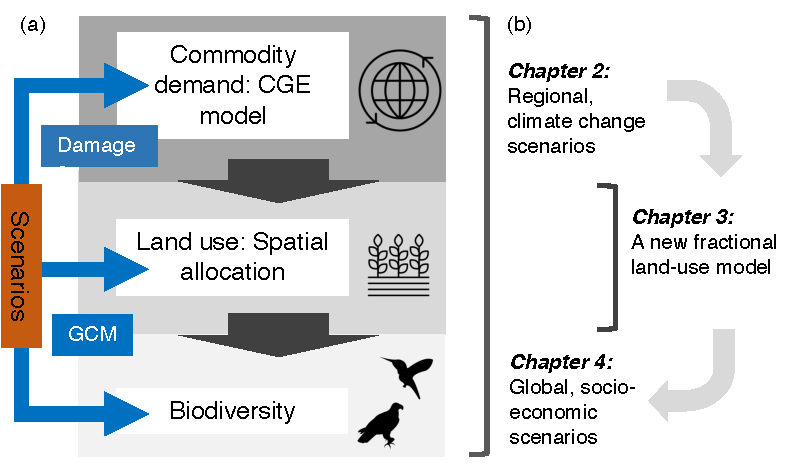
\includegraphics{chapters/figures/chapter1/fig_structure.pdf}
    \caption{Structure of this thesis in terms of the set-up of our framework. (a) Our modelling framework applying Computable General Equilibrium (CGE) models to predict commodity demand, land-use models to spatially downscale these demands and biodiversity models to predict biodiversity outcomes. Throughout our framework, scenarios have been parametrized through economic damages and general circulation models (GCM). (b) Thesis chapters in terms of the framework. Chapter 2 provides a first, regional implementation of our integrated assessment framework in which climate change impacts (RCP) are parametrized. Chapter 3 specifies a new fractional land-use model to improve the linkage of macro-economic and biodiversity models. Chapter 4 provides a first global implementation of our framework in which the new land-use model is first applied to spatially downscale SSP and predictions are compared to those made by an existing IAM. Adapted from \citet{kapitza_assessing_2021}.}
    \label{ch4:fig_structure}
\end{figure*}

\section{Chapter outline}

\subsection*{\Cref{ch2}: Assessing biophysical and socio-economic impacts of climate change on regional avian biodiversity}

The second chapter provides the initial development and application of our integrated assessment framework to quantify the relative influence of direct biophysical and indirect socio-economic (via commodity demand and land-use change) climate change impacts on bird species in Vietnam and Australia. In this chapter, we spatially downscaled projected changes in commodity demand using an existing categorical land-use model with limited applicability at global, fine-resolution extents.

\subsection*{\Cref{ch3}: A predictive model of fractional land use}
Resulting from \Cref{ch2}, we determined that in order to upscale our modelling framework to the global extent and align land-use predictions with the requirements posed by global-scale biodiversity modelling, it was necessary to develop a new fractional land-use model. In chapter 3 we introduce and validate a new land-use model to interface global commodity demand projections and biodiversity change. The model enables fine-scale mapping of future land-use under alternative scenarios of commodity demand change. It represents land-use as fractional cover within grid cells, thus providing higher information content than discrete categories of land-use without the need to decrease the spatial resolution.

\subsection*{\Cref{ch4}: Toward streamlined and transparent economic-ecological predictions of land-use change impacts on biodiversity}

Building on the methods and knowledge generated from \Cref{ch3,ch4}, the fourth chapter presents a first global implementation of our framework to predict global biodiversity nunder baseline SSP, thus paving the way for further analyses of climate change mitigation and adaptation scenarios on biodiversity. In this chapter, we parametrize baseline SSP in our CGE model and use the land-use model developed in chapter 3 to spatially downscale commodity demand change expected under SSP2 and SSP5. We also further extend our land-use model by implementing a method to predict land-use intensity. We apply biodiversity models to project biodiversity intactness. We compare land-use and biodiversity predictions made using our framework with those made using an existing ingegrated assessment model and demonstrate that our streamlined, simplified modelling framework provides a robust means to predict biodiversity change without the high parametrization requirements of existing integrated assessment frameworks.

\subsection*{\Cref{ch5}: General discussion}

This chapter provides synthesis of the main findings of thesis and relates them to the thesis aims. It includes a critical assessment of the developed methods in terms of their applicability outside of the project within which they were developed and their transferability to other study contexts. Future research potentials are highlighted.

\subsection*{Appendices}

\Cref{apx:ch2,apx:ch3,apx:ch4} contain all supplementary information for \Cref{ch2,ch3,ch4}. \Cref{apx:ch5} contains links to all \texttt{R} scripts written for this thesis and information about developed packages.
